% Name: Mealy machine
% Description: A Mealy machine that detects 101 in a bit stream, overlaps included: each edge is labeled input/output, and the output is 1 only on the edge that completes 101.
% Tags: Mealy machine, sequence detector, finite state machine, transducer

\usetikzlibrary{automata, arrows.meta}

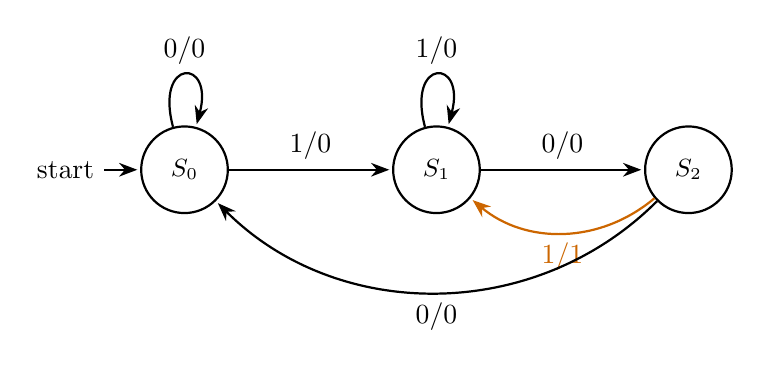
\begin{tikzpicture}[shorten >=1pt, auto, thick, >={Stealth}, every state/.style={minimum size=11mm, font=\small}]
  \node[state, initial] (s0) at (0,0) {$S_0$};
  \node[state] (s1) at (3.2,0) {$S_1$};
  \node[state] (s2) at (6.4,0) {$S_2$};
  % S0 has seen nothing useful, S1 a trailing 1, and S2 a trailing 10.
  \path[->]
    (s0) edge[loop above] node {$0/0$} ()
         edge node {$1/0$} (s1)
    (s1) edge[loop above] node {$1/0$} ()
         edge node {$0/0$} (s2)
    (s2) edge[bend left=40, orange!80!black] node {$1/1$} (s1)
         edge[bend left=45] node {$0/0$} (s0);
\end{tikzpicture}
